\section{Simulation}\label{sec:simulation}

\begin{figure}
\centering
\subfigure[Scenario 1]{
\qquad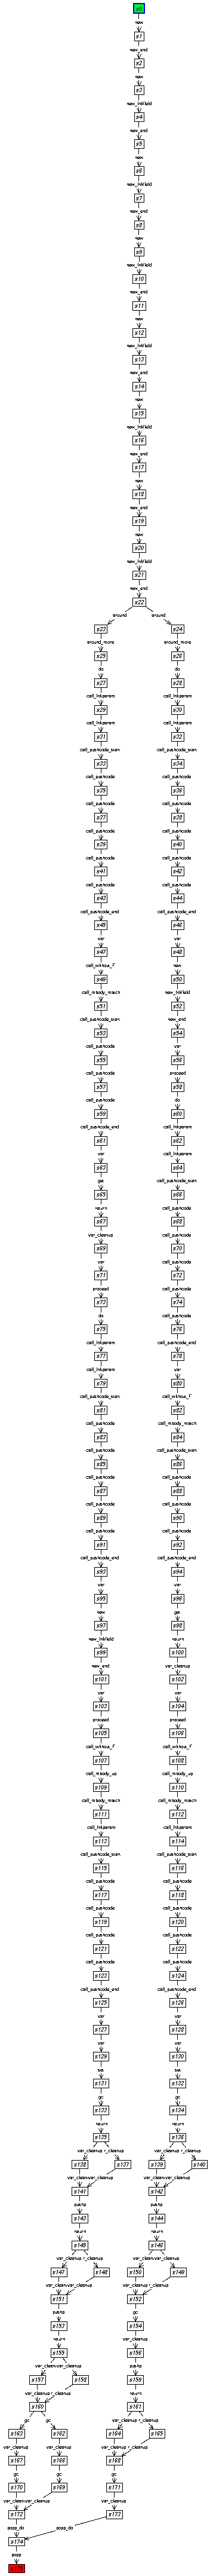
\includegraphics[scale=.07]{examples/lts5.png}\qquad
\label{fig:scenario1}
}\qquad
\subfigure[Scenario 2]{
\qquad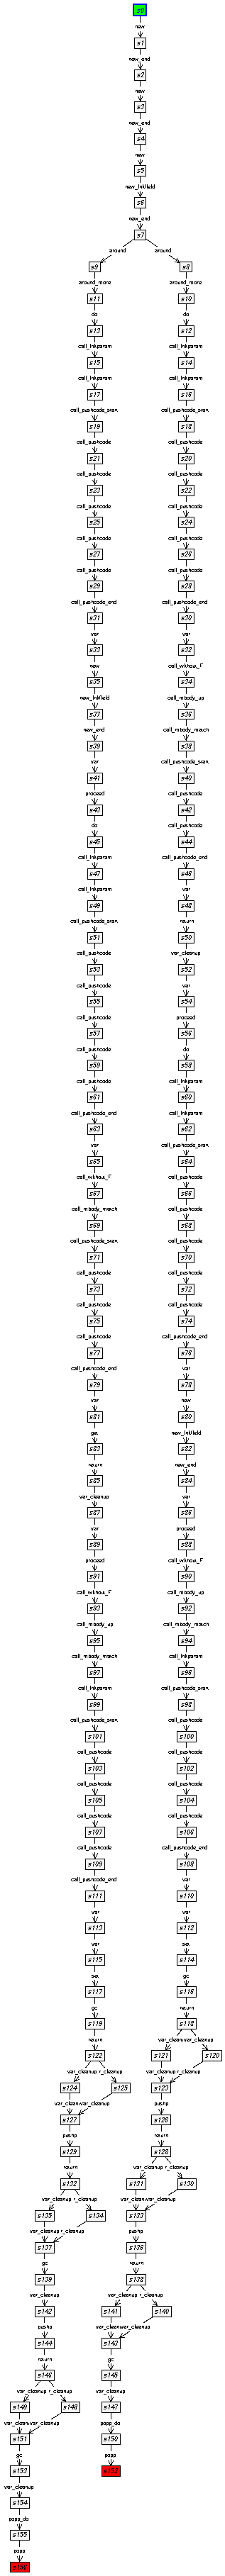
\includegraphics[scale=.07]{examples/lts0.png}\qquad
\label{fig:scenario2}
}
\caption{LTS for the Example Scenario's.}
\label{fig:lts_examples}
%{Caption of subfigures \subref{fig:subfig1}, \subref{fig:subfig2} and \subref{fig:subfig3}}
\end{figure}

We demonstrate the simulation capabilities of the semantics by means of the two scenarios of the example shown in Section \ref{sec:FAJ}. Simulation is done by using the GROOVE Simulator, which requires a graph production system and a start state. It will then try to match all rules in each state (while respecting any priorities). This results in an LTS, where states are graphs, and transitions are rule applications labelled the name of the applied rule. This provides a simple and intuitive visual representation of the execution of the simulated system, the LTS. This LTS can be used for analysis and verification, e.g. for model-checking.

Figure \ref{fig:lts_examples} show the generated LTS for the two scenarios. In Figure \ref{fig:scenario1}, the {\tt setGrade} method is called on an instance of {\tt NamedExam} with argument \emph{five}. The non-determinism at one-third visualises the two choices in scheduling the two advices. When, in both cases, the advices and the setGrade method have returned, the two branches merge into the same final result, where the grade is set to \emph{five}.
Figure \ref{fig:scenario2}, the argument of the {\tt setGrade} call is \emph{zero}, causing the second advice in the example to behave differently: zero decreased by one remains zero. Again, after one-third the LTS branches into the two scheduling scenarios. In the left branch, the first advice of the example is executed before the second advice, causing the final result to be {\tt zero} (it is first increased and then decreased). In the right branch, the second advice of the example is executed first, causing the final result to be \emph{one}. This is visualised by the two distinct final states: the branches are non-confluent. \\
